

\tikzset{every picture/.style={line width=0.75pt}} %set default line width to 0.75pt        

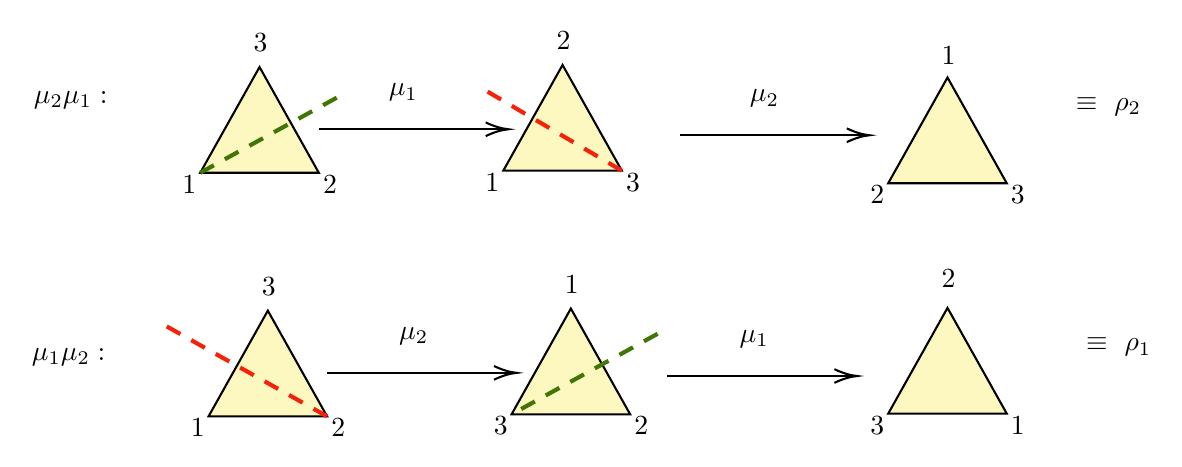
\begin{tikzpicture}[x=0.75pt,y=0.75pt,yscale=-1,xscale=1]
%uncomment if require: \path (0,227); %set diagram left start at 0, and has height of 227

%Straight Lines [id:da8577541306885849] 
\draw    (341.75,178.73) -- (431.12,178.73) ;
\draw [shift={(433.12,178.73)}, rotate = 180] [color={rgb, 255:red, 0; green, 0; blue, 0 }  ][line width=0.75]    (10.93,-3.29) .. controls (6.95,-1.4) and (3.31,-0.3) .. (0,0) .. controls (3.31,0.3) and (6.95,1.4) .. (10.93,3.29)   ;
%Straight Lines [id:da14363701357932668] 
\draw    (347.75,62.73) -- (437.12,62.73) ;
\draw [shift={(439.12,62.73)}, rotate = 180] [color={rgb, 255:red, 0; green, 0; blue, 0 }  ][line width=0.75]    (10.93,-3.29) .. controls (6.95,-1.4) and (3.31,-0.3) .. (0,0) .. controls (3.31,0.3) and (6.95,1.4) .. (10.93,3.29)   ;
%Shape: Triangle [id:dp6166967616717672] 
\draw  [fill={rgb, 255:red, 250; green, 238; blue, 106 }  ,fill opacity=0.43 ] (476.67,34.9) -- (505.22,85.84) -- (448.11,85.84) -- cycle ;
%Shape: Triangle [id:dp10184292255708727] 
\draw  [fill={rgb, 255:red, 250; green, 238; blue, 106 }  ,fill opacity=0.43 ] (476.67,145.9) -- (505.22,196.84) -- (448.11,196.84) -- cycle ;
%Shape: Triangle [id:dp16072718880753045] 
\draw  [fill={rgb, 255:red, 250; green, 238; blue, 106 }  ,fill opacity=0.43 ] (291.21,28.86) -- (319.76,79.8) -- (262.65,79.8) -- cycle ;

%Shape: Triangle [id:dp5648577801345768] 
\draw  [fill={rgb, 255:red, 250; green, 238; blue, 106 }  ,fill opacity=0.43 ] (145.21,29.86) -- (173.76,80.8) -- (116.65,80.8) -- cycle ;

%Straight Lines [id:da2701519616679303] 
\draw    (173.75,59.84) -- (263.12,59.84) ;
\draw [shift={(265.12,59.84)}, rotate = 180] [color={rgb, 255:red, 0; green, 0; blue, 0 }  ][line width=0.75]    (10.93,-3.29) .. controls (6.95,-1.4) and (3.31,-0.3) .. (0,0) .. controls (3.31,0.3) and (6.95,1.4) .. (10.93,3.29)   ;
%Straight Lines [id:da8423035151742334] 
\draw [color={rgb, 255:red, 65; green, 117; blue, 5 }  ,draw opacity=1 ][line width=1.5]  [dash pattern={on 5.63pt off 4.5pt}]  (116.65,80.8) -- (183,44.31) ;
%Shape: Triangle [id:dp6294228660813018] 
\draw  [fill={rgb, 255:red, 250; green, 238; blue, 106 }  ,fill opacity=0.43 ] (295.21,146.23) -- (323.76,197.17) -- (266.65,197.17) -- cycle ;

%Shape: Triangle [id:dp25618566511022456] 
\draw  [fill={rgb, 255:red, 250; green, 238; blue, 106 }  ,fill opacity=0.43 ] (149.21,147.23) -- (177.76,198.17) -- (120.65,198.17) -- cycle ;

%Straight Lines [id:da8827959373008387] 
\draw [color={rgb, 255:red, 247; green, 33; blue, 9 }  ,draw opacity=1 ][line width=1.5]  [dash pattern={on 5.63pt off 4.5pt}]  (177.76,198.17) -- (100,154.55) ;
%Straight Lines [id:da40930653904783754] 
\draw    (177.75,177.21) -- (267.12,177.21) ;
\draw [shift={(269.12,177.21)}, rotate = 180] [color={rgb, 255:red, 0; green, 0; blue, 0 }  ][line width=0.75]    (10.93,-3.29) .. controls (6.95,-1.4) and (3.31,-0.3) .. (0,0) .. controls (3.31,0.3) and (6.95,1.4) .. (10.93,3.29)   ;
%Straight Lines [id:da4786144067411211] 
\draw [color={rgb, 255:red, 247; green, 33; blue, 9 }  ,draw opacity=1 ][line width=1.5]  [dash pattern={on 5.63pt off 4.5pt}]  (319.76,79.8) -- (252,39.9) ;
%Straight Lines [id:da1460315703759597] 
\draw [color={rgb, 255:red, 65; green, 117; blue, 5 }  ,draw opacity=1 ][line width=1.5]  [dash pattern={on 5.63pt off 4.5pt}]  (337,158.38) -- (266.65,197.17) ;

% Text Node
\draw (34,164.12) node [anchor=north west][inner sep=0.75pt]    {$\mu _{1} \mu _{2} :$};
% Text Node
\draw (35,40.12) node [anchor=north west][inner sep=0.75pt]    {$\mu _{2} \mu _{1} :$};
% Text Node
\draw (375,155.4) node [anchor=north west][inner sep=0.75pt]    {$\mu _{1}$};
% Text Node
\draw (380,39.4) node [anchor=north west][inner sep=0.75pt]    {$\mu _{2}$};
% Text Node
\draw (438.03,85.64) node [anchor=north west][inner sep=0.75pt]    {$2$};
% Text Node
\draw (505.75,85.64) node [anchor=north west][inner sep=0.75pt]    {$3$};
% Text Node
\draw (472.3,18.44) node [anchor=north west][inner sep=0.75pt]    {$1$};
% Text Node
\draw (438.03,196.64) node [anchor=north west][inner sep=0.75pt]    {$3$};
% Text Node
\draw (505.75,196.64) node [anchor=north west][inner sep=0.75pt]    {$1$};
% Text Node
\draw (472.3,125.92) node [anchor=north west][inner sep=0.75pt]    {$2$};
% Text Node
\draw (206,36.51) node [anchor=north west][inner sep=0.75pt]    {$\mu _{1}$};
% Text Node
\draw (211,153.88) node [anchor=north west][inner sep=0.75pt]    {$\mu _{2}$};
% Text Node
\draw (537,42.97) node [anchor=north west][inner sep=0.75pt]    {$\equiv \ \rho _{2}$};
% Text Node
\draw (542,158.97) node [anchor=north west][inner sep=0.75pt]    {$\equiv \ \rho _{1}$};
% Text Node
\draw (144.84,129.77) node [anchor=north west][inner sep=0.75pt]    {$3$};
% Text Node
\draw (178.29,197.97) node [anchor=north west][inner sep=0.75pt]    {$2$};
% Text Node
\draw (110.57,197.97) node [anchor=north west][inner sep=0.75pt]    {$1$};
% Text Node
\draw (290.84,128.77) node [anchor=north west][inner sep=0.75pt]    {$1$};
% Text Node
\draw (324.29,196.97) node [anchor=north west][inner sep=0.75pt]    {$2$};
% Text Node
\draw (256.57,196.97) node [anchor=north west][inner sep=0.75pt]    {$3$};
% Text Node
\draw (140.84,12.4) node [anchor=north west][inner sep=0.75pt]    {$3$};
% Text Node
\draw (174.29,80.6) node [anchor=north west][inner sep=0.75pt]    {$2$};
% Text Node
\draw (106.57,80.6) node [anchor=north west][inner sep=0.75pt]    {$1$};
% Text Node
\draw (286.84,11.4) node [anchor=north west][inner sep=0.75pt]    {$2$};
% Text Node
\draw (320.29,79.6) node [anchor=north west][inner sep=0.75pt]    {$3$};
% Text Node
\draw (252.57,79.6) node [anchor=north west][inner sep=0.75pt]    {$1$};


\end{tikzpicture}
